\section{Parametric Equations}\label{sec:Parametric Equations}
When we computed the derivative $dy/dx$ using polar coordinates, we
used the expressions $x=f(\theta)\cos\theta$ and
$y=f(\theta)\sin\theta$. These two equations completely specify the
curve, though the form $r=f(\theta)$ is simpler. The expanded form has
the virtue that it can easily be generalized to describe a wider range
of curves than can be specified in rectangular or polar coordinates. 

Suppose $f(t)$ and $g(t)$ are functions. Then the equations
$x=f(t)$ and $y=g(t)$ describe a curve in the plane. In the case of
the polar coordinates equations, the variable $t$ is replaced by
$\theta$ which has a natural geometric interpretation. In general, $t$
is simply an arbitrary variable, often called in this case a
\dfont{parameter}\index{parameter}, and this method of specifying a curve is known as 
\dfont{parametric equations}\index{parametric equations}\index{polar coordinates!parametric equations}. One
important interpretation of $t$ is {\it time}. In this interpretation,
the equations $x=f(t)$ and $y=g(t)$ give the position of an object at
time $t$.

\begin{example}{Position of a Path}{positionofapath}
 Describe the path of an object that moves so that its
position at time $t$ is given by $x=\cos t$, $\ds y=\cos^2 t$.
\end{example}

\begin{solution}
We see immediately that $\ds y=x^2$, so the path lies on this parabola. The path
is not the entire parabola, however, since $x=\cos t$ is always
between $-1$ and $1$. It is now easy to see that the object oscillates
back and forth on the parabola between the endpoints $(1,1)$ and
$(-1,1)$, and is at point $(1,1)$ at time $t=0$.
\end{solution}

It is sometimes quite easy to describe a complicated path in
parametric equations when rectangular and polar coordinate expressions
are difficult or impossible to devise.

\begin{example}{Wheel}{wheelexample}
 A wheel of radius 1 rolls along a straight line, say the
$x$-axis. A point on the rim of the wheel will trace out a curve, called a
cycloid. Assume the point starts at the origin; find
parametric equations for the curve.
\end{example}

\begin{solution}
Figure~\ref{fig:cycloid} illustrates the generation of the curve. The wheel is shown at its
starting point, and again after it has rolled through about 490
degrees. We take as our parameter $t$ the angle through which the
wheel has turned, measured as shown clockwise from the line connecting
the center of the wheel to the ground. Since the radius is 1, the
center of the wheel has coordinates $(t,1)$. We seek to write the
coordinates of the point on the rim as $(t+\Delta x,1+\Delta y)$,
where $\Delta x$ and $\Delta y$ are as shown in figure~\ref{fig:blow
  up of wheel}. These values are nearly the sine and cosine of the
angle $t$, from the unit circle definition of sine and
cosine. However, some care is required because we are measuring $t$
from a nonstandard starting line and in a clockwise direction, as
opposed to the usual counterclockwise direction. A bit of thought
reveals that $\Delta x=-\sin t$ and $\Delta y=-\cos t$. Thus the
parametric equations for the cycloid are $x=t-\sin t$, $y=1-\cos t$.
\end{solution}

%
%\figure[!ht]
%\centerline{\vbox{\beginpicture
%\normalgraphs
%%\sevenpoint
%\setcoordinatesystem units <7truemm,7truemm>
%\setplotarea x from 0 to 20, y from 0  to 2.2
%\axis left shiftedto x=0 /
%\axis bottom shiftedto y=0 /
%\setquadratic
%\textRed
%\plot 0.000 0.000 0.001 0.018 0.009 0.070 0.030 0.156 0.069 0.271
%0.133 0.412 0.226 0.574 0.351 0.751 0.510 0.937 0.704 1.125
%0.934 1.309 1.197 1.482 1.491 1.637 1.813 1.771 2.157 1.876
%2.518 1.951 2.891 1.992 3.267 1.998 3.642 1.969 4.007 1.905
%4.358 1.809 4.687 1.685 4.991 1.536 5.265 1.368 5.506 1.187
%5.712 1.000 5.883 0.813 6.019 0.632 6.122 0.464 6.195 0.315
%6.243 0.191 6.269 0.095 6.281 0.031 6.283 0.002 6.284 0.008
%6.288 0.049 6.304 0.124 6.337 0.229 6.392 0.363 6.475 0.518
%6.589 0.691 6.736 0.875 6.919 1.063 7.137 1.249 7.389 1.426
%7.673 1.588 7.986 1.729 8.323 1.844 8.680 1.930 9.049 1.982
%9.425 2.000 9.801 1.982 10.170 1.930 10.526 1.844 10.863 1.729
%11.176 1.588 11.461 1.426 11.713 1.249 11.931 1.063 12.113 0.875
%12.261 0.691 12.375 0.518 12.457 0.363 12.513 0.229 12.545 0.124
%12.561 0.049 12.566 0.008 12.566 0.002 12.569 0.031 12.580 0.095
%12.607 0.191 12.654 0.315 12.727 0.464 12.830 0.632 12.966 0.813
%13.137 1.000 13.343 1.187 13.584 1.368 13.858 1.536 14.162 1.685
%14.492 1.809 14.842 1.905 15.208 1.969 15.582 1.998 15.959 1.992
%16.331 1.951 16.692 1.876 17.037 1.771 17.358 1.637 17.652 1.482
%17.916 1.309 18.145 1.125 18.340 0.937 18.499 0.751 18.623 0.574
%18.716 0.412 18.780 0.271 18.820 0.156 18.841 0.070 18.848 0.018
%18.850 0.000 /
%\textBlack
%\plot 8.500 0.800 8.442 0.799 8.383 0.816 8.329 0.850 8.286 0.900
%8.258 0.962 8.248 1.033 8.259 1.105 8.291 1.174 8.343 1.233
%8.412 1.277 8.493 1.299 8.579 1.298 8.664 1.272 8.740 1.221
%8.800 1.150 8.839 1.061 8.851 0.963 8.835 0.863 8.791 0.769
%8.720 0.690 8.627 0.632 8.520 0.602 8.406 0.604 8.294 0.638
%8.195 0.704 8.116 0.797 8.066 0.910 8.049 1.036 8.068 1.164
%8.124 1.283 /
%\multiput {$\bullet$} at 0 0 7.70 1.602 /
%\put {$t$} [bl] <2pt,2pt> at 8.73 1.23
%\setlinear
%\plot 7.70 1.602 8.5 1 8.5 0 /
%\circulararc 360 degrees from 0 0 center at 0 1 
%\circulararc 360 degrees from 8.5 0 center at 8.5 1
%\endpicture}}
%\caption{{A cycloid.} \label{fig:cycloid}}
%\endfigure

\figure[H]
\[
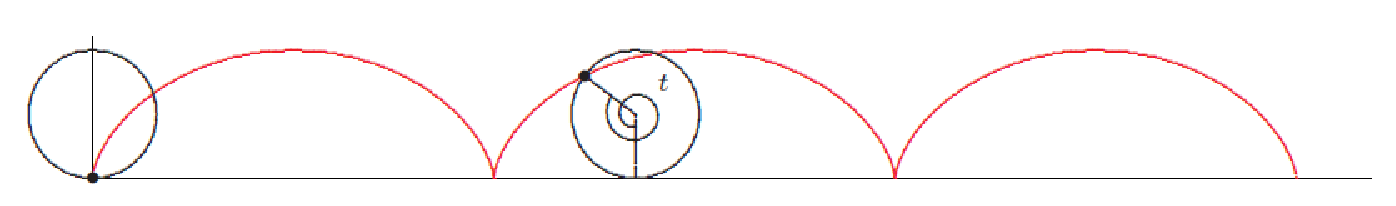
\includegraphics[width=4.5in]{images/7-cycloid} 
\] 
\caption{{A cycloid.} \label{fig:cycloid}}
\endfigure

\figure[H]
\centerline{\vbox{\beginpicture
\normalgraphs
%\sevenpoint
\setcoordinatesystem units <15truemm,15truemm>
\setplotarea x from -1 to 1, y from 0 to 2
\multiput {$\bullet$} at -0.8 1.602 /
%\plot 0.000 0.800 -0.058 0.799 -0.117 0.816 -0.171 0.850 -0.214 0.900
%-0.242 0.962 -0.252 1.033 -0.241 1.105 -0.209 1.174 -0.157 1.233
%-0.088 1.277 -0.007 1.299 0.079 1.298 0.164 1.272 0.240 1.221
%0.300 1.150 0.339 1.061 0.351 0.963 0.335 0.863 0.291 0.769
%0.220 0.690 0.127 0.632 0.020 0.602 -0.094 0.604 -0.206 0.638
%-0.305 0.704 -0.384 0.797 -0.434 0.910 -0.451 1.036 -0.432 1.164
%-0.376 1.283 /
\putrule from -0.8 1.602 to -0.8 1
\putrule from -0.8 1 to 0 1
\put {$\Delta x$} [t] <0pt,-2pt> at -0.4 1
\put {$\Delta y$} [l] <2pt,0pt> at -0.8 1.2
\setlinear
\plot -0.8 1.602 0 1 0 0 /
\circulararc 360 degrees from 0 0 center at 0 1
\endpicture}}
\caption{{The wheel.} \label{fig:blow up of wheel}}
\endfigure



%%%%%%%%%%%%%%%%%%%%%%%%%%%%%%%%%%%%%%%%%%%%
\Opensolutionfile{solutions}[ex]
\section*{Exercises for \ref{sec:Parametric Equations}}

\begin{enumialphparenastyle}

%%%%%%%%%%
\begin{ex}
 What curve is described by $\ds x=t^2$, $\ds y=t^4$? If $t$ is
interpreted as time, describe how the object moves on the curve.
\end{ex}

%%%%%%%%%%
\begin{ex}
 What curve is described by $x=3\cos t$, $y=3\sin t$? If $t$ is
interpreted as time, describe how the object moves on the curve.
\end{ex}

%%%%%%%%%%
\begin{ex}
 What curve is described by $x=3\cos t$, $y=2\sin t$? If $t$ is
interpreted as time, describe how the object moves on the curve.
\end{ex}

%%%%%%%%%%
\begin{ex}
 What curve is described by $x=3\sin t$, $y=3\cos t$? If $t$ is
interpreted as time, describe how the object moves on the curve.
\end{ex}

%%%%%%%%%%
\begin{ex}
 Sketch the curve described by $\ds x=t^3-t$, $\ds y=t^2$. If $t$ is
interpreted as time, describe how the object moves on the curve.
\end{ex}

%%%%%%%%%%%
\begin{ex}\label{exer:pseudo cycloid}
 A wheel of radius 1 rolls along a straight line, say the
$x$-axis. A point $P$ is located halfway between the center of the
wheel and the rim; assume $P$ starts at the point $(0,1/2)$. As the
wheel rolls, $P$ traces a curve; find parametric equations for the
curve.
\begin{sol}
 $\ds x=t-{\sin(t)\over2}$, $\ds t=1-{\cos(t)\over2}$
\end{sol}
\end{ex}

%%%%%%%%%%%
%\\begin{ex}
% A wheel of radius 1 rolls around the outside of a circle of
%radius 3. A point $P$ on the rim of the wheel traces out a curve
%called a \dfont{hypercycloid}, as indicated in
%figure~\ref{fig:hypercycloid and hypocycloid}.  Assuming $P$
%starts at the point $(3,0)$, find parametric equations for the curve.
%\begin{sol}
% $x=4\cos t-\cos(4t)$,\hfill\break  $y=4\sin t-\sin(4t)$
%\end{sol}
%\end{ex}
%\exrdef{exer:hypercycloid}
%
%\figure
%\vbox{\beginpicture
%\normalgraphs
%\sevenpoint
%\setcoordinatesystem units <7truemm,7truemm>
%\setplotarea x from -5 to 5, y from -5  to 5
%\axis left shiftedto x=0 /
%\axis bottom shiftedto y=0 /
%\multiput {$\bullet$} at 2.81 4.12 3 0 /
%\circulararc 360 degrees from 2.81 4.12 center at 2.16 3.366
%\circulararc 360 degrees from 0 3 center at 0 0
%\circulararc 360 degrees from 5 0 center at 4 0
%\textRed
%\setquadratic
%\plot 3.000 0.000 3.024 0.002 3.092 0.020 3.200 0.065 3.339 0.150
%3.495 0.285 3.656 0.474 3.807 0.721 3.931 1.022 4.015 1.373
%4.045 1.763 4.012 2.182 3.908 2.613 3.730 3.041 3.479 3.450
%3.160 3.824 2.781 4.148 2.353 4.410 1.890 4.602 1.410 4.717
%0.927 4.755 0.459 4.719 0.021 4.614 -0.375 4.450 -0.717 4.241
%-1.000 4.000 -1.220 3.743 -1.378 3.487 -1.478 3.245 -1.531 3.030
%-1.545 2.853 -1.535 2.721 -1.516 2.637 -1.501 2.600 -1.506 2.607
%-1.542 2.648 -1.620 2.714 -1.746 2.791 -1.924 2.864 -2.152 2.918
%-2.427 2.939 -2.740 2.914 -3.079 2.832 -3.432 2.685 -3.782 2.471
%-4.113 2.187 -4.410 1.839 -4.658 1.434 -4.845 0.983 -4.961 0.500
%-5.000 0.000 -4.961 -0.500 -4.845 -0.983 -4.658 -1.434 -4.410 -1.839
%-4.113 -2.187 -3.782 -2.471 -3.432 -2.685 -3.079 -2.832 -2.740 -2.914
%-2.427 -2.939 -2.152 -2.918 -1.924 -2.864 -1.746 -2.791 -1.620 -2.714
%-1.542 -2.648 -1.506 -2.607 -1.501 -2.600 -1.516 -2.637 -1.535 -2.721
%-1.545 -2.853 -1.531 -3.030 -1.478 -3.245 -1.378 -3.487 -1.220 -3.743
%-1.000 -4.000 -0.717 -4.241 -0.375 -4.450 0.021 -4.614 0.459 -4.719
%0.927 -4.755 1.410 -4.717 1.890 -4.602 2.353 -4.410 2.781 -4.148
%3.160 -3.824 3.479 -3.450 3.730 -3.041 3.908 -2.613 4.012 -2.182
%4.045 -1.763 4.015 -1.373 3.931 -1.022 3.807 -0.721 3.656 -0.474
%3.495 -0.285 3.339 -0.150 3.200 -0.065 3.092 -0.020 3.024 -0.002
%3.000 0.000 /
%\textBlack
%\setcoordinatesystem units <7truemm,7truemm> point at -12 0
%\setplotarea x from -3.5 to 3.5, y from -3.5  to 3.5
%\axis left shiftedto x=0 /
%\axis bottom shiftedto y=0 /
%\multiput {$\bullet$} at 3 0 /
%%\circulararc 360 degrees from 2.81 4.12 center at 2.16 3.366
%\circulararc 360 degrees from 0 3 center at 0 0
%\circulararc 360 degrees from 3 0 center at 2 0
%\textRed
%\setquadratic
%\plot 3.000 0.000 2.985 0.000 2.942 0.003 2.870 0.009 2.771 0.021
%2.645 0.041 2.496 0.070 2.325 0.110 2.134 0.161 1.927 0.225
%1.706 0.301 1.474 0.390 1.234 0.492 0.989 0.606 0.744 0.731
%0.500 0.866 0.261 1.010 0.030 1.160 -0.191 1.314 -0.399 1.471
%-0.592 1.628 -0.769 1.781 -0.928 1.929 -1.067 2.069 -1.187 2.197
%-1.287 2.312 -1.367 2.410 -1.427 2.490 -1.469 2.549 -1.492 2.586
%-1.500 2.598 -1.493 2.585 -1.473 2.546 -1.443 2.481 -1.404 2.389
%-1.358 2.270 -1.309 2.127 -1.258 1.959 -1.207 1.768 -1.158 1.557
%-1.113 1.327 -1.074 1.081 -1.043 0.823 -1.019 0.554 -1.005 0.279
%-1.000 0.000 -1.005 -0.279 -1.019 -0.554 -1.043 -0.823 -1.074 -1.081
%-1.113 -1.327 -1.158 -1.557 -1.207 -1.768 -1.258 -1.959 -1.309 -2.127
%-1.358 -2.270 -1.404 -2.389 -1.443 -2.481 -1.473 -2.546 -1.493 -2.585
%-1.500 -2.598 -1.492 -2.586 -1.469 -2.549 -1.427 -2.490 -1.367 -2.410
%-1.287 -2.312 -1.187 -2.197 -1.067 -2.069 -0.928 -1.929 -0.769 -1.781
%-0.592 -1.628 -0.399 -1.471 -0.191 -1.314 0.030 -1.160 0.261 -1.010
%0.500 -0.866 0.744 -0.731 0.989 -0.606 1.234 -0.492 1.474 -0.390
%1.706 -0.301 1.927 -0.225 2.134 -0.161 2.325 -0.110 2.496 -0.070
%2.645 -0.041 2.771 -0.021 2.870 -0.009 2.942 -0.003 2.985 -0.000
%3.000 0.000 /
%\textBlack
%\endpicture}
%\label{fig:hypercycloid and hypocycloid}
%\endfigure{A hypercycloid and a hypocycloid.}
%
%
%%%%%%%%%%%
%\\begin{ex}
% A wheel of radius 1 rolls around the inside of 
%a circle of radius 3. A point $P$ on the rim of the wheel traces out a
%curve called a \dfont{hypocycloid}, as indicated in
%figure~\ref{fig:hypercycloid and hypocycloid}. Assuming $P$
%starts at the point $(3,0)$, find parametric equations for the curve.
%\begin{sol}
% $x=2\cos t+\cos(2t)$,\hfill\break $y=2\sin t-\sin(2t)$
%\end{sol}
%\end{ex}
%\exrdef{exer:hypocycloid}
%
%%%%%%%%%%%
%\\begin{ex}
% An \dfont{involute\index{involute}} of a circle is formed
%as follows: Imagine that a long (that is, infinite) string is wound tightly
%around a circle, and that you grasp the end of the string and begin to
%unwind it, keeping the string taut. The end of the string traces out
%the involute. Find parametric equations for this curve, using a circle
%of radius 1, and assuming that the string unwinds counter-clockwise
%and the end of the string is initially at $(1,0)$. 
%Figure~\ref{fig:involute} shows part of the curve; the
%dotted lines represent the string at a few different times.
%\begin{sol}
% $x=\cos t+t\sin t$,\hfill\break  $y=\sin t-t\cos t$
%\end{sol}
%\end{ex}
%\exrdef{exer:involute of a circle}
%
%\figure
%\vbox{\beginpicture
%\normalgraphs
%\sevenpoint
%\setcoordinatesystem units <7truemm,7truemm>
%\setplotarea x from -5 to 2, y from -4  to 3.5
%\axis left shiftedto x=0 /
%\axis bottom shiftedto y=0 /
%\circulararc 360 degrees from 0 1 center at 0 0
%\setquadratic
%\textRed
%\plot 1.000 0.000 1.002 0.000 1.008 0.001 1.018 0.002 1.031 0.005
%1.048 0.010 1.069 0.018 1.092 0.028 1.118 0.041 1.147 0.058
%1.178 0.079 1.211 0.105 1.245 0.135 1.280 0.170 1.315 0.210
%1.350 0.255 1.385 0.306 1.418 0.362 1.449 0.423 1.478 0.490
%1.504 0.563 1.527 0.640 1.545 0.723 1.559 0.811 1.568 0.903
%1.571 1.000 1.568 1.101 1.558 1.205 1.541 1.312 1.516 1.422
%1.484 1.534 1.443 1.647 1.393 1.761 1.335 1.875 1.268 1.989
%1.191 2.102 1.105 2.212 1.010 2.320 0.905 2.425 0.791 2.526
%0.668 2.621 0.536 2.711 0.395 2.794 0.246 2.870 0.088 2.939
%-0.077 2.998 -0.250 3.048 -0.429 3.088 -0.614 3.117 -0.805 3.135
%-1.000 3.142 -1.199 3.135 -1.402 3.116 -1.606 3.084 -1.812 3.038
%-2.019 2.978 -2.225 2.903 -2.430 2.815 -2.632 2.712 -2.831 2.594
%-3.025 2.462 -3.214 2.316 -3.396 2.155 -3.570 1.981 -3.736 1.793
%-3.892 1.592 -4.037 1.378 -4.171 1.152 -4.292 0.914 -4.399 0.666
%-4.492 0.408 -4.570 0.141 -4.631 -0.135 -4.676 -0.417 -4.703 -0.706
%-4.712 -1.000 -4.703 -1.298 -4.675 -1.598 -4.627 -1.901 -4.559 -2.203
%-4.472 -2.504 -4.364 -2.803 -4.236 -3.099 -4.088 -3.389 -3.920 -3.672 /
%%-3.733 -3.948 
%%-3.526 -4.215 -3.300 -4.471 -3.056 -4.715 -2.794 -4.946
%%-2.515 -5.163 -2.219 -5.363 -1.908 -5.547 -1.583 -5.713 -1.244 -5.860
%%-0.893 -5.986 -0.531 -6.091 -0.160 -6.174 0.220 -6.234 0.607 -6.271
%%1.000 -6.283 /
%\textBlack
%\setlinear\setdashes <2pt>
%\plot 0.54 0.84 1.38 0.3 /
%\plot -0.65 -0.757 -3.68 1.86 /
%\plot -0.42 0.91 1.4 1.74 /
%\endpicture}
%\label{fig:involute}
%\endfigure{An involute of a circle.}
%
%\end%%%%%%%%%%
%\\begin{ex}
%s

\end{enumialphparenastyle}
